\chapter{Introduction}

\startcontents[chapters]
% \printmyminitoc{

% }

 Ensuring customer satisfaction stands as one of the most important goals for enterprises across industries. Customer satisfaction is a term frequently used in marketing. It is a measure of how products and services supplied by a company meet or surpass customer expectations. Customer satisfaction is defined as "the number of customers, or percentage of total customers, whose reported experience with a firm, its products, or its services (ratings) exceeds specified satisfaction goals."\cite{cus_sas} Customers play an important role and are essential in keeping a product or service relevant, so it is, therefore, in the best interest of the business to ensure customer satisfaction and build customer loyalty. 

\begin{figure}[H]
    \centering
    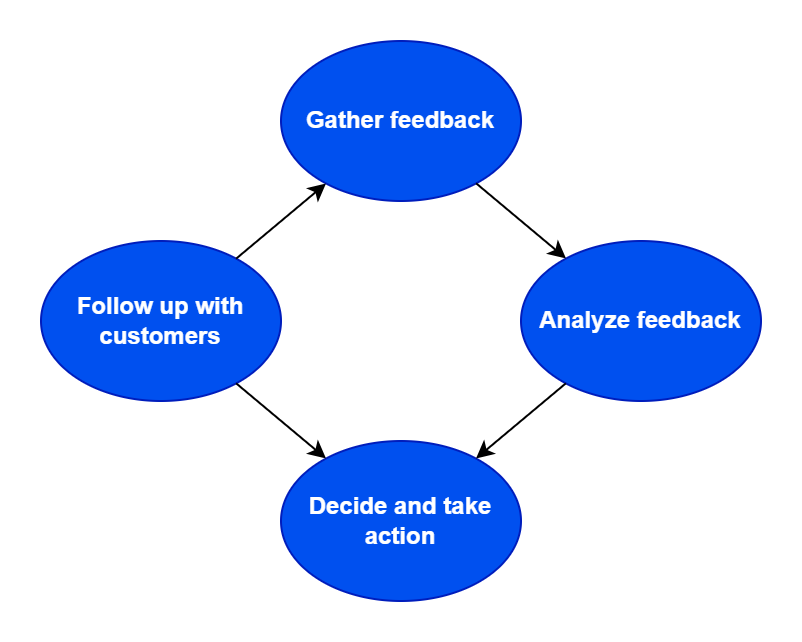
\includegraphics[width=0.7\textwidth]{images/customer-sastifaction.drawio.png}
    \caption{Customer satisfaction loop}
    \label{fig:cus_satis}
\end{figure}

With fierce competition in today's market, the collection and analysis of invaluable data derived from customer interactions is the key to improving companies' competitive advantage. Analysis of customer calls to the call center by using NLP techniques to distill meaning from these interactions and extract actionable insights is also one of the missions that the company takes place to improve customer relationships and heighten service quality.

To achieve this objective, I use NLP techniques to cluster the recorded phone calls of the customer with the SFR call center. Central to this approach is the utilization of CamemBERT\cite{martin2020camembert}—a specialized French language model and variant of the RoBERTa\cite{liu2019roberta} architecture. CamemBERT is leveraged to transform the linguistic essence of each sentence into a vector within a vector space. These vectors serve as a representation of the meaning of each sentence. After that, I will apply some clustering techniques in these transformed vectors, thus discovering the most important words of each cluster by using TF-IDF, a technique to extract pivotal keywords, and the most representative documents closely aligned with centroids.

The objective is to use the most significant word of each topic as a suggestion for the call team, who need to determine the topic of calls manually. By suggesting the words and the topics for the team, it could be easier to label topics for the call, as well as the labeling process will be more accurate and suggest the labelers to labels that he or she does not have enough time to describe a conversation and select all relevant tags fully.